\chapter{Echinodermata, Hemichordata and
Chordata}\label{echinodermata-hemichordata-and-chordata}

\href{https://en.wikipedia.org/wiki/Echinoderm}{Echinodermata} (the
phylum which includes starfish, sea urchins, sea cucumbers, and
crinoids) and
\href{https://en.wikipedia.org/wiki/Hemichordate}{Hemichordata}, form
the \href{https://en.wikipedia.org/wiki/Ambulacraria}{ambulacraria}, the
sister taxon of the chordates. The
\href{https://en.wikipedia.org/wiki/Chordate}{Chordata} and ambulacraria
form the superphylum deuterostomia, composed of the deuterostomes.
Deuterostomes are one of the two major divisions of the bilaterians, the
other being the protostomes. During the early development of the embryo,
in deuterostomes, the blastopore (the first opening to form) becomes the
anus whereas in the protostomes, it becomes the mouth. In deuterostomes,
the mouth develops at a later stage, at the opposite end of the blastula
from the blastopore, and a gut forms connecting the two.

\section{Echinodermata}\label{echinodermata}

Echinoderm is the common name given to any member of the phylum
Echinodermata (from Ancient Greek, echinos -- ``hedgehog'' and derma --
``skin'') of marine animals. The adults are recognizable by their
(usually five-point) radial symmetry, and include such well-known
animals as sea stars, sea urchins, sand dollars, and sea cucumbers, as
well as the sea lilies or ``stone lilies''. Echinoderms are found at
every ocean depth, from the intertidal zone to the abyssal zone. The
phylum contains about 7000 living species, making it the second-largest
grouping of deuterostomes (a superphylum), after the chordates (which
include the vertebrates, such as birds, fishes, mammals, and reptiles).
Echinoderms are also the largest phylum that has no freshwater or
terrestrial (land-based) representatives.

The first definitive members of the phylum appeared near the start of
the Cambrian. One group of Cambrian echinoderms, the cinctans
(Homalozoa), which are close to the base of the echinoderm origin, have
been found to possess external gills used for filter feeding, like
Chordata and Hemichordata.

The echinoderms are important both ecologically and geologically.
Ecologically, there are few other groupings so abundant in the biotic
desert of the deep sea, as well as shallower oceans. Most echinoderms
are able to regenerate tissue, organs, limbs, and reproduce asexually;
in some cases, they can undergo complete regeneration from a single
limb. Geologically, the value of echinoderms is in their ossified
skeletons, which are major contributors to many limestone formations,
and can provide valuable clues as to the geological environment. They
were the most used species in regenerative research in the 19th and 20th
centuries.

Along with the chordates and hemichordates, echinoderms are
deuterostomes, one of the two major divisions of the bilaterians, the
other being the protostomes. During the early development of the embryo,
in deuterostomes, the blastopore (the first opening to form) becomes the
anus whereas in the protostomes, it becomes the mouth. In deuterostomes,
the mouth develops at a later stage, at the opposite end of the blastula
from the blastopore, and a gut forms connecting the two. The larvae of
echinoderms have bilateral symmetry but this is lost during
metamorphosis when their bodies are reorganized and develop the
characteristic radial symmetry of the echinoderm, typically pentamerism
(literally: consisting of 5 parts). The characteristics of adult
echinoderms are the possession of a water vascular system with external
tube feet and a calcareous endoskeleton consisting of ossicles connected
by a mesh of collagen fibres.

Two main subdivisions are traditionally recognized:

\begin{enumerate}
\def\labelenumi{\arabic{enumi}.}
\tightlist
\item
  Eleutherozoa, which encompasses the Asteroidea (starfish), Ophiuroidea
  (brittle stars), Echinoidea (sea urchins and sand dollars) and
  Holothuroidea (sea cucumbers).
\item
  Pelmatozoa, some of which are sessile while others move around. These
  consist of the Crinoidea (feather stars and sea lilies).
\end{enumerate}

Echinoderms have a mesodermal skeleton composed of calcareous plates or
ossicles. Each one of these, even the articulating spine of a sea
urchin, is composed mineralogically of a crystal of calcite. If solid,
these would form a heavy skeleton, so they have a sponge-like porous
structure known as stereom. Ossicles may be fused together, as in the
test of sea urchins, or may articulate with each other as in the arms of
sea stars, brittle stars and crinoids. The ossicles may be flat plates
or bear external projections in the form of spines, granules or warts
and they are supported by a tough epidermis (skin). Skeletal elements
are also deployed in some specialized ways, such as the ``Aristotle's
lantern'' mouthparts of sea urchins used for grinding, the supportive
stalks of crinoids and the structural ``lime ring'' of sea cucumbers.

The epidermis consists of cells responsible for the support and
maintenance of the skeleton, as well as pigment cells, mechanoreceptor
cells (which detect motion on the animal's surface), and sometimes gland
cells which secrete sticky fluids or even toxins. The varied and often
vivid colors of echinoderms are produced by the action of skin pigment
cells.

Echinoderms possess a unique water vascular system. This is a network of
fluid-filled canals derived from the coelom (body cavity) that function
in gas exchange, feeding, sensory reception and locomotion. This system
varies between different classes of echinoderm but typically opens to
the exterior through a sieve-like madreporite on the aboral (upper)
surface of the animal. The madreporite is linked to a slender duct, the
stone canal, which extends to a ring canal that encircles the mouth or
esophagus. From this, radial canals extend along the arms of asteroids
and adjoin the test in the ambulacral areas of echinoids. Short lateral
canals branch off the radial canals, each one ending in an ampulla. Part
of the ampulla can protrude through a pore (or a pair of pores in sea
urchins) to the exterior and is known as a podium or tube feet. The
water vascular system assists with the distribution of nutrients
throughout the animal's body and is most obviously expressed in the tube
feet which can be extended or contracted by the redistribution of fluid
between the foot and the internal sac.

Echinoderms possess a simple digestive system which varies according to
the animal's diet. Starfish are mostly carnivorous and have a mouth,
esophagus, two-part stomach, intestine and rectum, with the anus located
in the center of the aboral body surface. In many species, the large
cardiac stomach can be everted and digest food outside the body. In
other species, whole food items such as mollusks may be ingested.
Brittle stars have a blind gut with no intestine or anus. They have
varying diets and expel food waste through their mouth. Sea urchins are
herbivores and use their specialized mouthparts to graze, tear and chew
algae and sometimes other animal or vegetable material. They have an
esophagus, a large stomach and a rectum with the anus at the apex of the
test. Sea cucumbers are mostly detritivores, sorting through the
sediment with their buccal tentacles which are modified tube feet. Sand
and mud accompanies their food through their simple gut which has a
long, coiled intestine and a capacious cloaca. Crinoids are passive
suspension feeders, catching plankton with their outstretched arms.
Boluses of mucus-trapped food are passed to the mouth which is linked to
the anus by a loop consisting of a short esophagus and longer intestine.

The coelomic cavities of echinoderms are complex. Aside from the water
vascular system, echinoderms have a haemal coelom (or haemal system, the
``haemal'' being a misnomer), a perivisceral coelom, a gonadal coelom
and often also a perihaemal coelom (or perihaemal system). The water
vascular system, haemal system and perihaemal system form the tubular
coelomic system. Echinoderms are an exception having both a coelomic
circulatory system (i.e., the water vascular system) and a haemal
circulatory system (i.e., the haemal and perihaemal systems). Haemal and
perihaemal systems are derived from the coelom and form an open and
reduced circulatory system. This usually consists of a central ring and
five radial vessels. There is no true heart and the blood often lacks
any respiratory pigment. Gaseous exchange occurs via dermal branchae or
papulae in starfish, genital bursae in brittle stars, peristominal gills
in sea urchins and cloacal trees in sea cucumbers. Exchange of gases
also takes place through the tube feet. Echinoderms lack specialized
excretory (waste disposal) organs and so nitrogenous waste, chiefly in
the form of ammonia, diffuses out through the respiratory surfaces.

Echinoderms have a simple radial nervous system that consists of a
modified nerve net consisting of interconnecting neurons with no central
brain, although some do possess ganglia. Nerves radiate from central
rings around the mouth into each arm or along the body wall; the
branches of these nerves coordinate the movements of the organism and
the synchronization of the tube feet. Starfish have sensory cells in the
epithelium and have simple eyespots and touch-sensitive tentacle-like
tube feet at the tips of their arms. Sea urchins have no particular
sense organs but do have statocysts that assist in gravitational
orientation, and they have sensory cells in their epidermis,
particularly in the tube feet, spines and pedicellariae. Brittle stars,
crinoids and sea cucumbers in general do not have sensory organs but
some burrowing sea cucumbers of the order Apodida have a single
statocyst adjoining each radial nerve and some have an eyespot at the
base of each tentacle.

The gonads occupy much of the body cavities of sea urchins and sea
cucumbers, while the less voluminous crinoids, brittle stars and
starfish have two gonads in each arm. While the ancestral condition is
considered to be the possession of one genital aperture, many organisms
have multiple gonopores through which eggs or sperm may be released.

\section{Starfish}\label{starfish}

\href{https://en.wikipedia.org/wiki/Starfish}{Starfish} or sea stars are
star-shaped echinoderms belonging to the class Asteroidea. Common usage
frequently finds these names being also applied to ophiuroids, which are
correctly referred to as brittle stars or ``basket stars''. About 1,500
species of starfish occur on the seabed in all the world's oceans, from
the tropics to frigid polar waters. They are found from the intertidal
zone down to abyssal depths, 6,000 m below the surface.

Starfish are marine invertebrates. They typically have a central disc
and five arms, though some species have a larger number of arms. The
aboral or upper surface may be smooth, granular or spiny, and is covered
with overlapping plates. Many species are brightly colored in various
shades of red or orange, while others are blue, grey or brown. Starfish
have tube feet operated by a hydraulic system and a mouth at the center
of the oral or lower surface. They are opportunistic feeders and are
mostly predators on benthic invertebrates. Several species have
specialized feeding behaviors including eversion of their stomachs and
suspension feeding. They have complex life cycles and can reproduce both
sexually and asexually. Most can regenerate damaged parts or lost arms
and they can shed arms as a means of defense. The Asteroidea occupy
several significant ecological roles. Starfish, such as the ochre sea
star (Pisaster ochraceus) and the reef sea star (Stichaster australis),
have become widely known as examples of the keystone species concept in
ecology. The tropical crown-of-thorns starfish (\emph{Acanthaster planci}) is a
voracious predator of coral throughout the Indo-Pacific region, and the
northern Pacific sea star is considered to be one of the world's 100
worst invasive species.

The fossil record for starfish is ancient, dating back to the Ordovician
around 450 million years ago, but it is rather poor, as starfish tend to
disintegrate after death. Only the ossicles and spines of the animal are
likely to be preserved, making remains hard to locate. With their
appealing symmetrical shape, starfish have played a part in literature,
legend, design and popular culture.

\subsection{Sexual reproduction}\label{sexual-reproduction-1}

Most species of starfish are
\href{https://en.wikipedia.org/wiki/Gonochorism}{gonochorous},
i.e.~there are separate male and female individuals. These are usually
not distinguishable externally as the gonads cannot be seen, but their
sex is apparent when they spawn. Some species are simultaneous
hermaphrodites, producing eggs and sperm at the same time and in a few
of these, the same gonad, called an ovotestis, produces both eggs and
sperm. Other starfish are sequential hermaphrodites. Protandrous
individuals of species like Asterina gibbosa start life as males before
changing sex into females as they grow older. In some species such as
\emph{Nepanthia belcheri}, a large female can split in half and the resulting
offspring are males. When these grow large enough they change back into
females. The lifespan of a starfish varies considerably between species,
generally being longer in larger forms and in those with planktonic
larvae (up to lifespan more than 30 years).

Some species of starfish have the ability to regenerate lost arms and
can regrow an entire new limb given time. A few can regrow a complete
new disc from a single arm, while others need at least part of the
central disc to be attached to the detached part. Regrowth can take
several months or years, and starfish are vulnerable to infections
during the early stages after the loss of an arm.

Each starfish arm contains two gonads that release gametes through
openings called gonoducts, located on the central disc between the arms.
Fertilization is generally external but in a few species, internal
fertilization takes place. In most species, the buoyant eggs and sperm
are simply released into the water (free spawning) and the resulting
embryos and larvae live as part of the plankton. In others, the eggs may
be stuck to the undersides of rocks. In certain species of starfish, the
females brood their eggs -- either by simply enveloping them or by
holding them in specialized structures. In brooding species, the eggs
are relatively large, and supplied with yolk, and they generally develop
directly into miniature starfish without an intervening larval stage.
The developing young are called lecithotrophic because they obtain their
nutrition from the yolk as opposed to ``planktotrophic'' larvae that
feed in the water column.

In the tropics, a plentiful supply of phytoplankton is continuously
available for starfish larvae to feed on. Spawning takes place at any
time of year, each species having its own characteristic breeding
season. In temperate regions, the spring and summer brings an increase
in food supplies. The first individual of a species to spawn may release
a pheromone that serves to attract other starfish to aggregate and to
release their gametes synchronously. In other species, a male and female
may come together and form a pair. This behavior is called
pseudocopulation and the male climbs on top, placing his arms between
those of the female. When she releases eggs into the water, he is
induced to spawn. Starfish may use environmental signals to coordinate
the time of spawning (day length to indicate the correct time of the
year, dawn or dusk to indicate the correct time of day), and chemical
signals to indicate their readiness to breed. In some species, mature
females produce chemicals to attract sperm in the sea water.

Some species of starfish are able to reproduce asexually as adults
either by fission of their central discs or by autotomy of one or more
of their arms.

Most starfish embryos hatch at the blastula stage. The original ball of
cells develops a lateral pouch, the archenteron. The entrance to this is
known as the blastopore and it will later develop into the anus. Another
invagination of the surface will fuse with the tip of the archenteron as
the mouth while the interior section will become the gut. At the same
time, a band of cilia develops on the exterior. This enlarges and
extends around the surface and eventually onto two developing arm-like
outgrowths. At this stage, the larva is known as a bipinnaria. The cilia
are used for locomotion and feeding, their rhythmic beat wafting
phytoplankton towards the mouth.

The next stage in development is a brachiolaria larva and involves the
growth of three short, additional arms. These are at the anterior end,
surround a sucker and have adhesive cells at their tips. Both bipinnaria
and brachiolaria larvae are bilaterally symmetrical. When fully
developed, the brachiolaria settles on the seabed and attaches itself
with a short stalk formed from the ventral arms and sucker.
Metamorphosis now takes place with a radical rearrangement of tissues.
The left side of the larval body becomes the oral surface of the
juvenile and the right side the aboral surface. Part of the gut is
retained but the mouth and anus move to new positions. Some of the body
cavities degenerate but others become the water vascular system and the
visceral coelom. The starfish is now pentaradially symmetrical. It casts
off its stalk and becomes a free-living juvenile starfish about 1 mm in
diameter.

\section{Starfish Dissection}\label{perform-starfish-dissection}

\begin{enumerate}
\def\labelenumi{\arabic{enumi}.}
\tightlist
\item
  Get a dissecting pan, scissors and a pointer.
\item
  Obtain a preserved starfish.
\item
  Place the starfish in the dissecting pan with its dorsal or aboral
  (top) surface upward.
\item
  Locate the central disc in the center of the starfish. Count and
  record the number of arms or rays the starfish has.
\item
  Locate the small, round hard plate called the madreporite on top of
  the central disc. Water enters through this into the water vascular
  system.
\item
  Feel the upper surface of the starfish for spines. These spines
  protect the starfish and are part of their endoskeleton.
\item
  Turn the starfish over to its ventral or oral surface.
\item
  Locate the mouth in the center of the central disc. Find the ring of
  oral spines surrounding the mouth.
\item
  Find the groove that extends down the underside of each arm. This is
  called the ambulacral groove.
\item
  Feel the numerous, soft tube feet inside each groove. The tube feet
  are part of the water vascular system and aid in movement and feeding.
\item
  With the starfish's aboral surface facing you, choose three rays and
  cut off the tip of each ray.
\item
  Cut along each side of each ray towards the central disc and then
  carefully remove the flap of skin (Fig. \ref{fig:starfish}.
\item
  Inside each arm, locate two long digestive glands called the pyloric
  caeca. These make enzymes to digest food in the stomach.
\item
  Cut a circular flap of skin from the central disc. (You will have to
  also cut around the madreporite in order to remove this flap.) Observe
  the stomach under the central disc.
\item
  Remove the pyloric caeca from one of the dissected rays.
\item
  Find the gonads (testes or ovaries) underneath. These may be small if
  the starfish is NOT in breeding season.
\item
  In the third ray, remove both the pyloric cecae and the gonads to see
  the water vascular system. Embedded in the soft body wall are skeletal
  plates called ossicles.
\item
  Cut off the tip of a ray to observe the parts of the tube feet. Find
  the zipper-like ridge that extends the length of the ray. The tube
  feet are attached to these.
\item
  Locate the bulb-like top of a tube foot called the ampulla. This sac
  works like the top of an eyedropper to create suction. The bottom of
  the tube foot is a sucker.
\end{enumerate}

\begin{figure}

{\centering 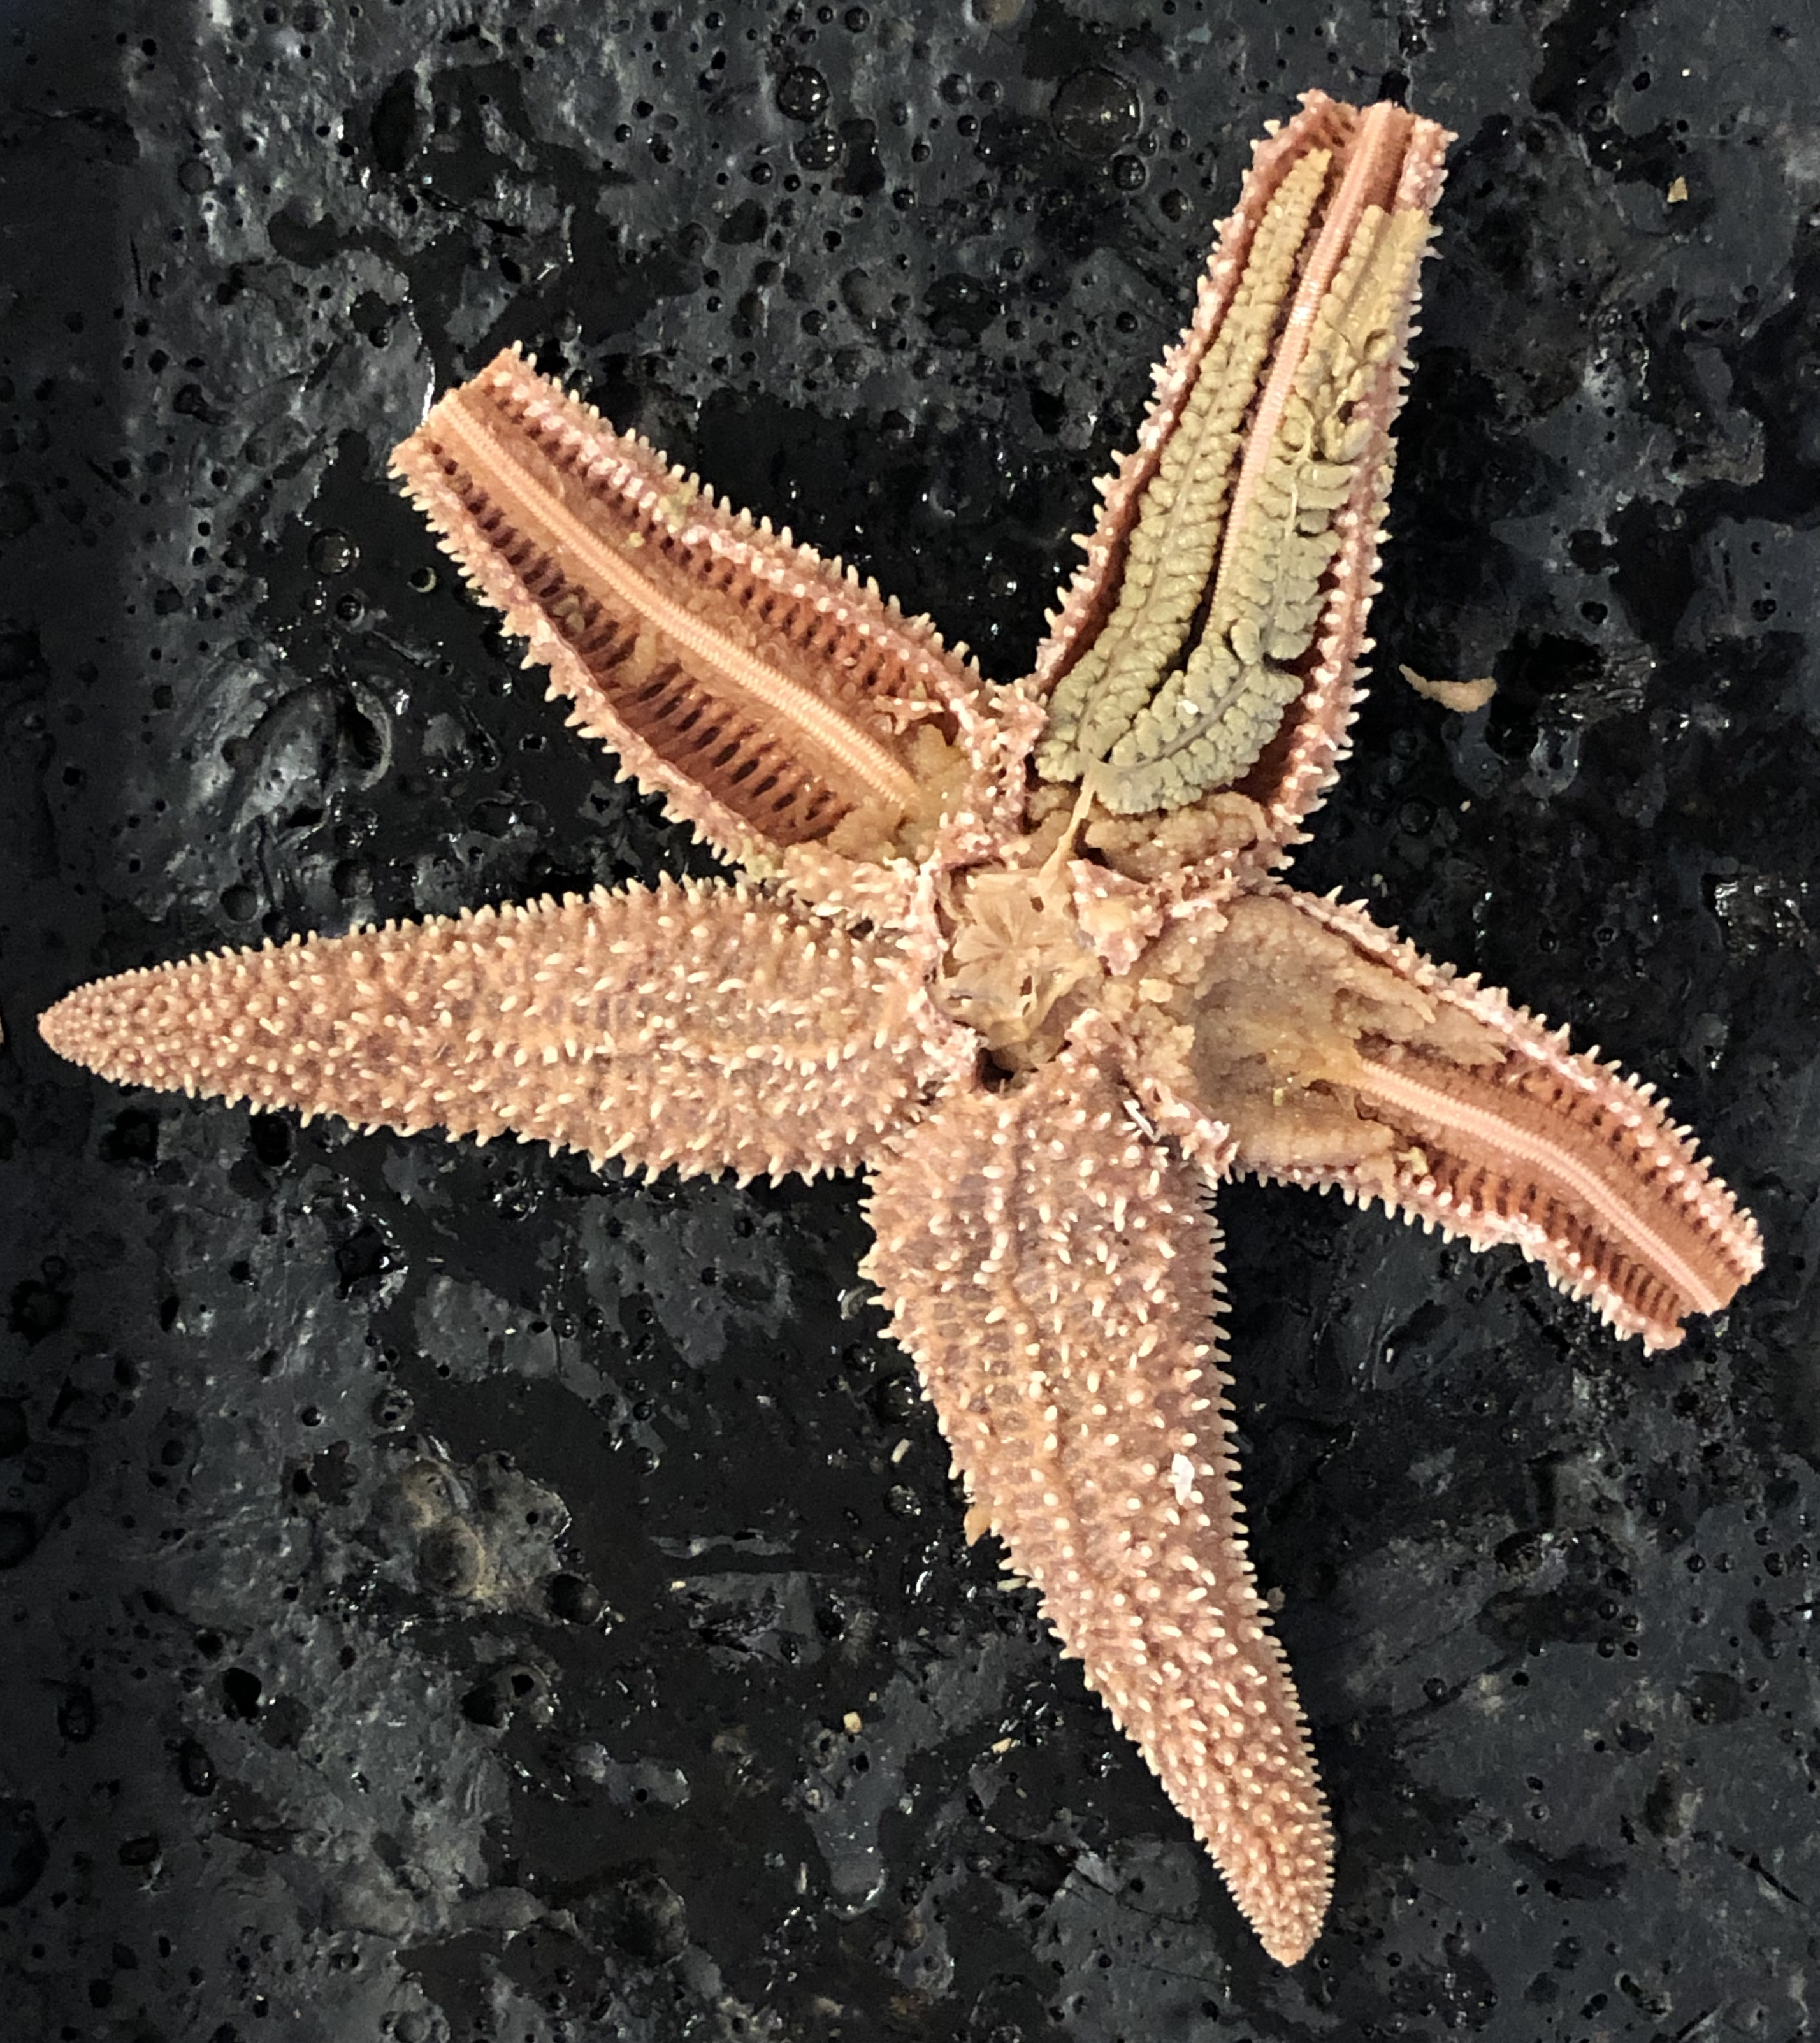
\includegraphics[width=0.7\linewidth]{./figures/echinodermata/starfish}

}

\caption{Starfish with exposed pyloric cecae, gonads and ambulacral ridge.}\label{fig:starfish}
\end{figure}

\section{View Prepared Slides of
Asterias}\label{view-prepared-slides-of-asterias}

\begin{enumerate}
\def\labelenumi{\arabic{enumi}.}
\tightlist
\item
  Starfish tube feet (Figure \ref{fig:tubefeet})

  \begin{itemize}
  \tightlist
  \item
    Locate: tube feet, suckers
  \end{itemize}
\item
  Asterias pedicellariae w.m. (Figure \ref{fig:pedicellariae})

  \begin{itemize}
  \tightlist
  \item
    Locate: pincer-like structures used to cleanse the skin.
  \end{itemize}
\end{enumerate}

\begin{figure}

{\centering 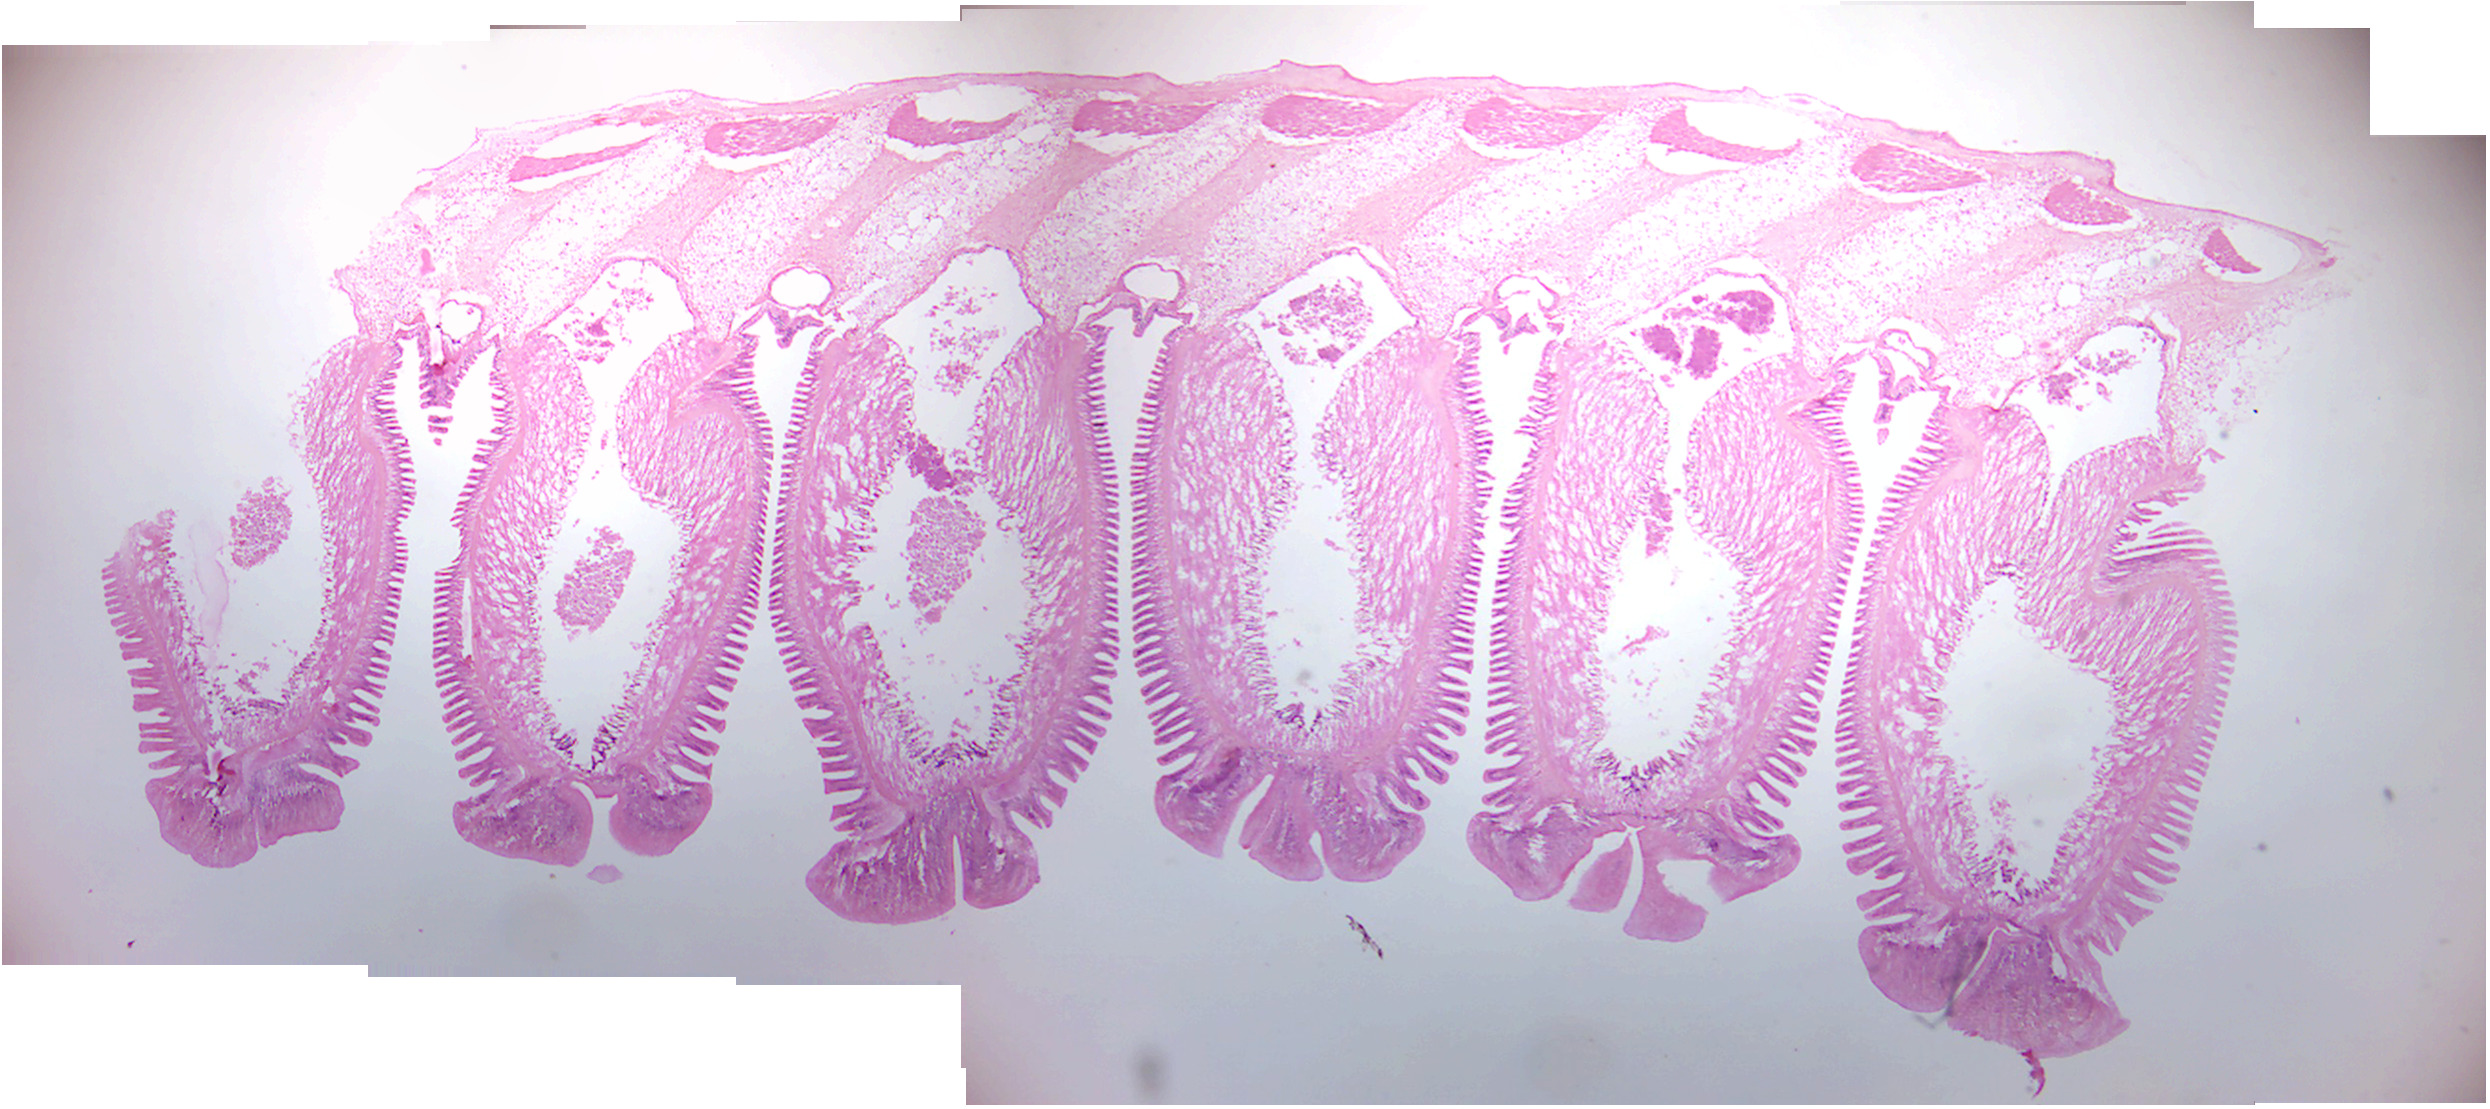
\includegraphics[width=0.7\linewidth]{./figures/echinodermata/starfish_tubefeet}

}

\caption{Starfish tube feet.}\label{fig:tubefeet}
\end{figure}

\begin{figure}

{\centering 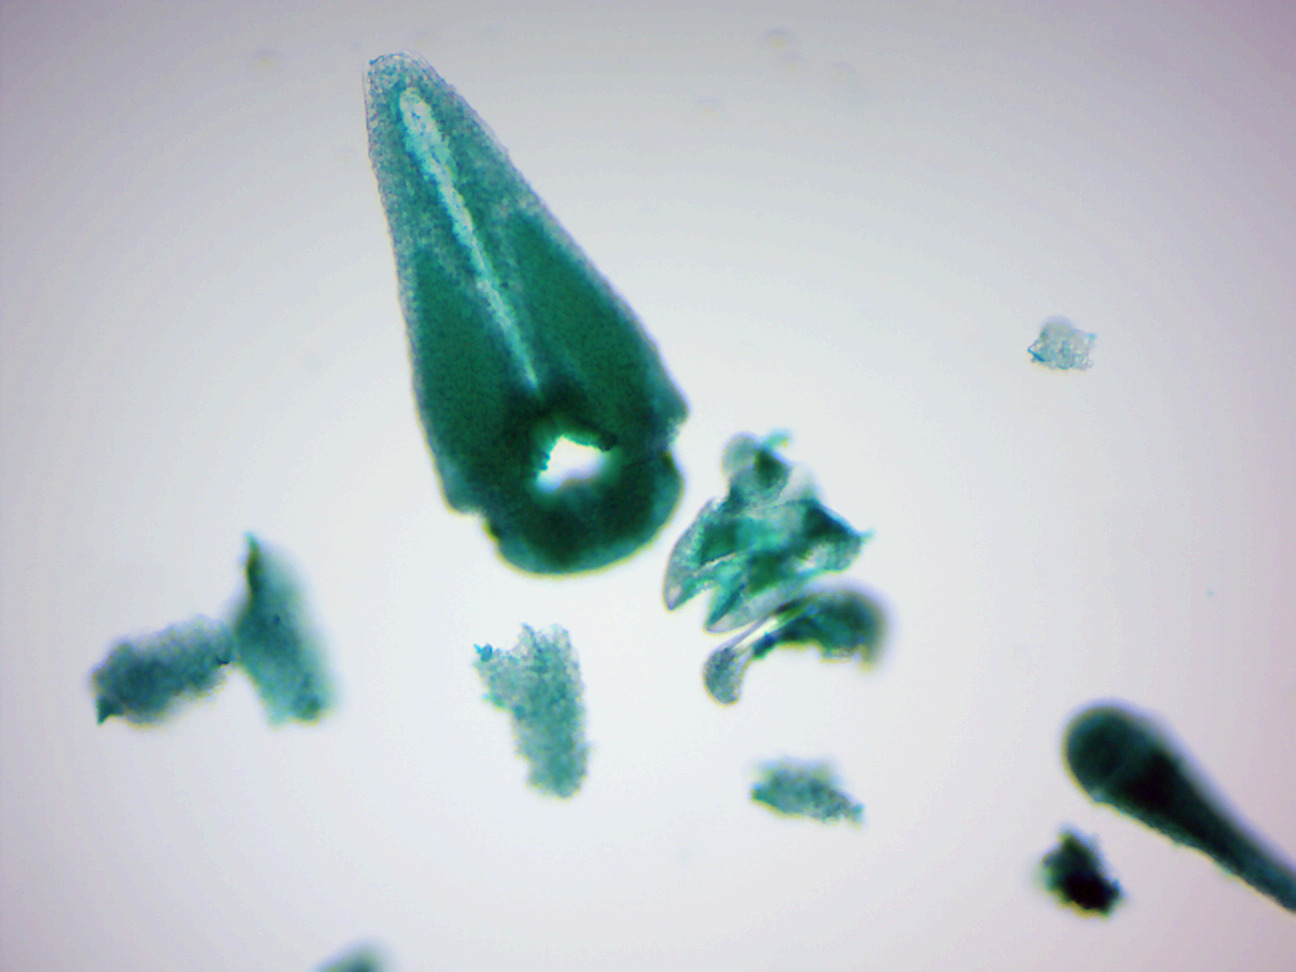
\includegraphics[width=0.7\linewidth]{./figures/echinodermata/pedicellariae}

}

\caption{Starfish pedicellariae.}\label{fig:pedicellariae}
\end{figure}

\section{Hemichordata}\label{hemichordata}

\href{https://en.wikipedia.org/wiki/Hemichordate}{Hemichordata} is a
phylum of marine deuterostome animals, generally considered the sister
group of the echinoderms. They appear in the Lower or Middle Cambrian
and include two main classes: Enteropneusta (acorn worms), and
Pterobranchia. A third class, Planctosphaeroidea, is known only from the
larva of a single species, Planctosphaera pelagica.

Acorn worms are solitary worm-shaped organisms. They generally live in
burrows (the earliest secreted tubes) and are deposit feeders, but some
species are pharyngeal filter feeders, while the family Torquaratoridae
are free living detritivores. Many are well known for their production
and accumulation of various halogenated phenols and pyrroles.
Pterobranchs are filter-feeders, mostly colonial, living in a
collagenous tubular structure called a coenecium.

The body of acorn worms is worm-shaped and divided into an anterior
proboscis, an intermediate collar, and a posterior trunk. The proboscis
is a muscular and ciliated organ used in locomotion and in the
collection and transport of food particles. The mouth is located between
the proboscis and the collar. The trunk is the longest part of the
animal. It contains the pharynx, which is perforated with gill slits (or
pharyngeal slits), the esophagus, a long intestine, and a terminal anus.
It also contains the gonads.

\section{Chordata}\label{chordata}

A chordate is an animal belonging to the phylum
\href{https://en.wikipedia.org/wiki/Chordate}{Chordata}; chordates
possess a notochord, a hollow dorsal nerve cord, pharyngeal slits, an
endostyle, and a muscular post-anal tail, for at least some period of
their life cycle. Chordates are deuterostomes, as during the embryo
development stage the anus forms before the mouth. They are also
bilaterally symmetric coelomates with metameric segmentation and a
circulatory system. In the case of vertebrate chordates, the notochord
is usually replaced by a vertebral column during development.

Taxonomically, the phylum includes the following subphyla:

\begin{itemize}
\tightlist
\item
  Vertebrata, which includes fish, amphibians, reptiles, birds, and
  mammals
\item
  Tunicata, which includes salps and sea squirts
\item
  Cephalochordata, which include the lancelets
\end{itemize}

Of the more than 65,000 living species of chordates, about half are bony
fish of the superclass Osteichthyes (boney fish). The world's largest
and fastest animals, the blue whale and peregrine falcon respectively,
are chordates, as are humans. Fossil chordates are known from at least
as early as the Cambrian explosion.

Chordates form a phylum of animals that are defined by having at some
stage in their lives all of the following:

\begin{itemize}
\tightlist
\item
  A notochord, a fairly stiff rod of cartilage that extends along the
  inside of the body. Among the vertebrate sub-group of chordates, the
  notochord develops into the spine, and in wholly aquatic species this
  helps the animal to swim by flexing its tail.
\item
  A dorsal neural tube. In fish and other vertebrates, this develops
  into the spinal cord, the main communications trunk of the nervous
  system
\item
  Pharyngeal slits. The pharynx is the part of the throat immediately
  behind the mouth. In fish, the slits are modified to form gills, but
  in some other chordates they are part of a filter-feeding system that
  extracts particles of food from the water in which the animals live.
\item
  Post-anal tail. A muscular tail that extends backwards behind the
  anus.
\item
  An endostyle. This is a groove in the ventral wall of the pharynx. In
  filter-feeding species it produces mucus to gather food particles,
  which helps in transporting food to the esophagus. It also stores
  iodine, and may be a precursor of the vertebrate thyroid gland.
\end{itemize}

There are soft constraints that separate chordates from certain other
biological lineages, but have not yet been made part of the formal
definition:

\begin{itemize}
\tightlist
\item
  All chordates are deuterostomes. This means that, during the embryo
  development stage, the anus forms before the mouth.
\item
  All chordates are based on a bilateral body plan.
\item
  All chordates are coelomates, and have a fluid filled body cavity
  called a coelom with a complete lining called peritoneum derived from
  mesoderm (see Brusca and Brusca).
\end{itemize}

\section{Craniata (Vertebrata)}\label{craniata-vertebrata}

Craniates, one of the three subdivisions of chordates, all have distinct
skulls. They include the hagfish which have no vertebrae. Michael J.
Benton commented that ``craniates are characterized by their heads, just
as chordates, or possibly all deuterostomes, are by their tails''.

Most are vertebrates, in which the notochord is replaced by the
vertebral column. These consist of a series of bony or cartilaginous
cylindrical vertebrae, generally with neural arches that protect the
spinal cord, and with projections that link the vertebrae. However,
hagfish have incomplete braincases and no vertebrae, and are therefore
not regarded as vertebrates, but as members of the craniates, the group
from which vertebrates are thought to have evolved. However, the
cladistic exclusion of hagfish from the vertebrates is controversial, as
they may be degenerate vertebrates who have lost their vertebral
columns.

The position of lampreys is ambiguous. They have complete braincases and
rudimentary vertebrae, and therefore may be regarded as vertebrates and
true fish. However, molecular phylogenetics, which uses biochemical
features to classify organisms, has produced both results that group
them with vertebrates and others that group them with hagfish. If
lampreys are more closely related to the hagfish than the other
vertebrates, this would suggest that they form a clade, which has been
named the Cyclostomata (literally: round mouths).

\section{Tunicates}\label{tunicates}

Most \href{https://en.wikipedia.org/wiki/Tunicate}{tunicates} appear as
adults in two major forms, both of which are soft-bodied filter-feeders
that lack the standard features of chordates: ``sea squirts'' are
sessile and consist mainly of water pumps and filter-feeding apparatus;
salps float in mid-water, feeding on plankton, and have a two-generation
cycle in which one generation is solitary and the next forms chain-like
colonies. However, all tunicate larvae have the standard chordate
features, including long, tadpole-like tails; they also have rudimentary
brains, light sensors and tilt sensors. The third main group of
tunicates, Appendicularia (also known as Larvacea) retain tadpole-like
shapes and active swimming all their lives, and were for a long time
regarded as larvae of sea squirts or salps. The etymology of the term
Urochorda(ta) (Balfour 1881) is from the ancient Greek oura, ``tail'') +
Latin chorda (``cord''), because the notochord is only found in the
tail. The term Tunicata (Lamarck 1816) is recognized as having
precedence and is now more commonly used.

\begin{figure}

{\centering 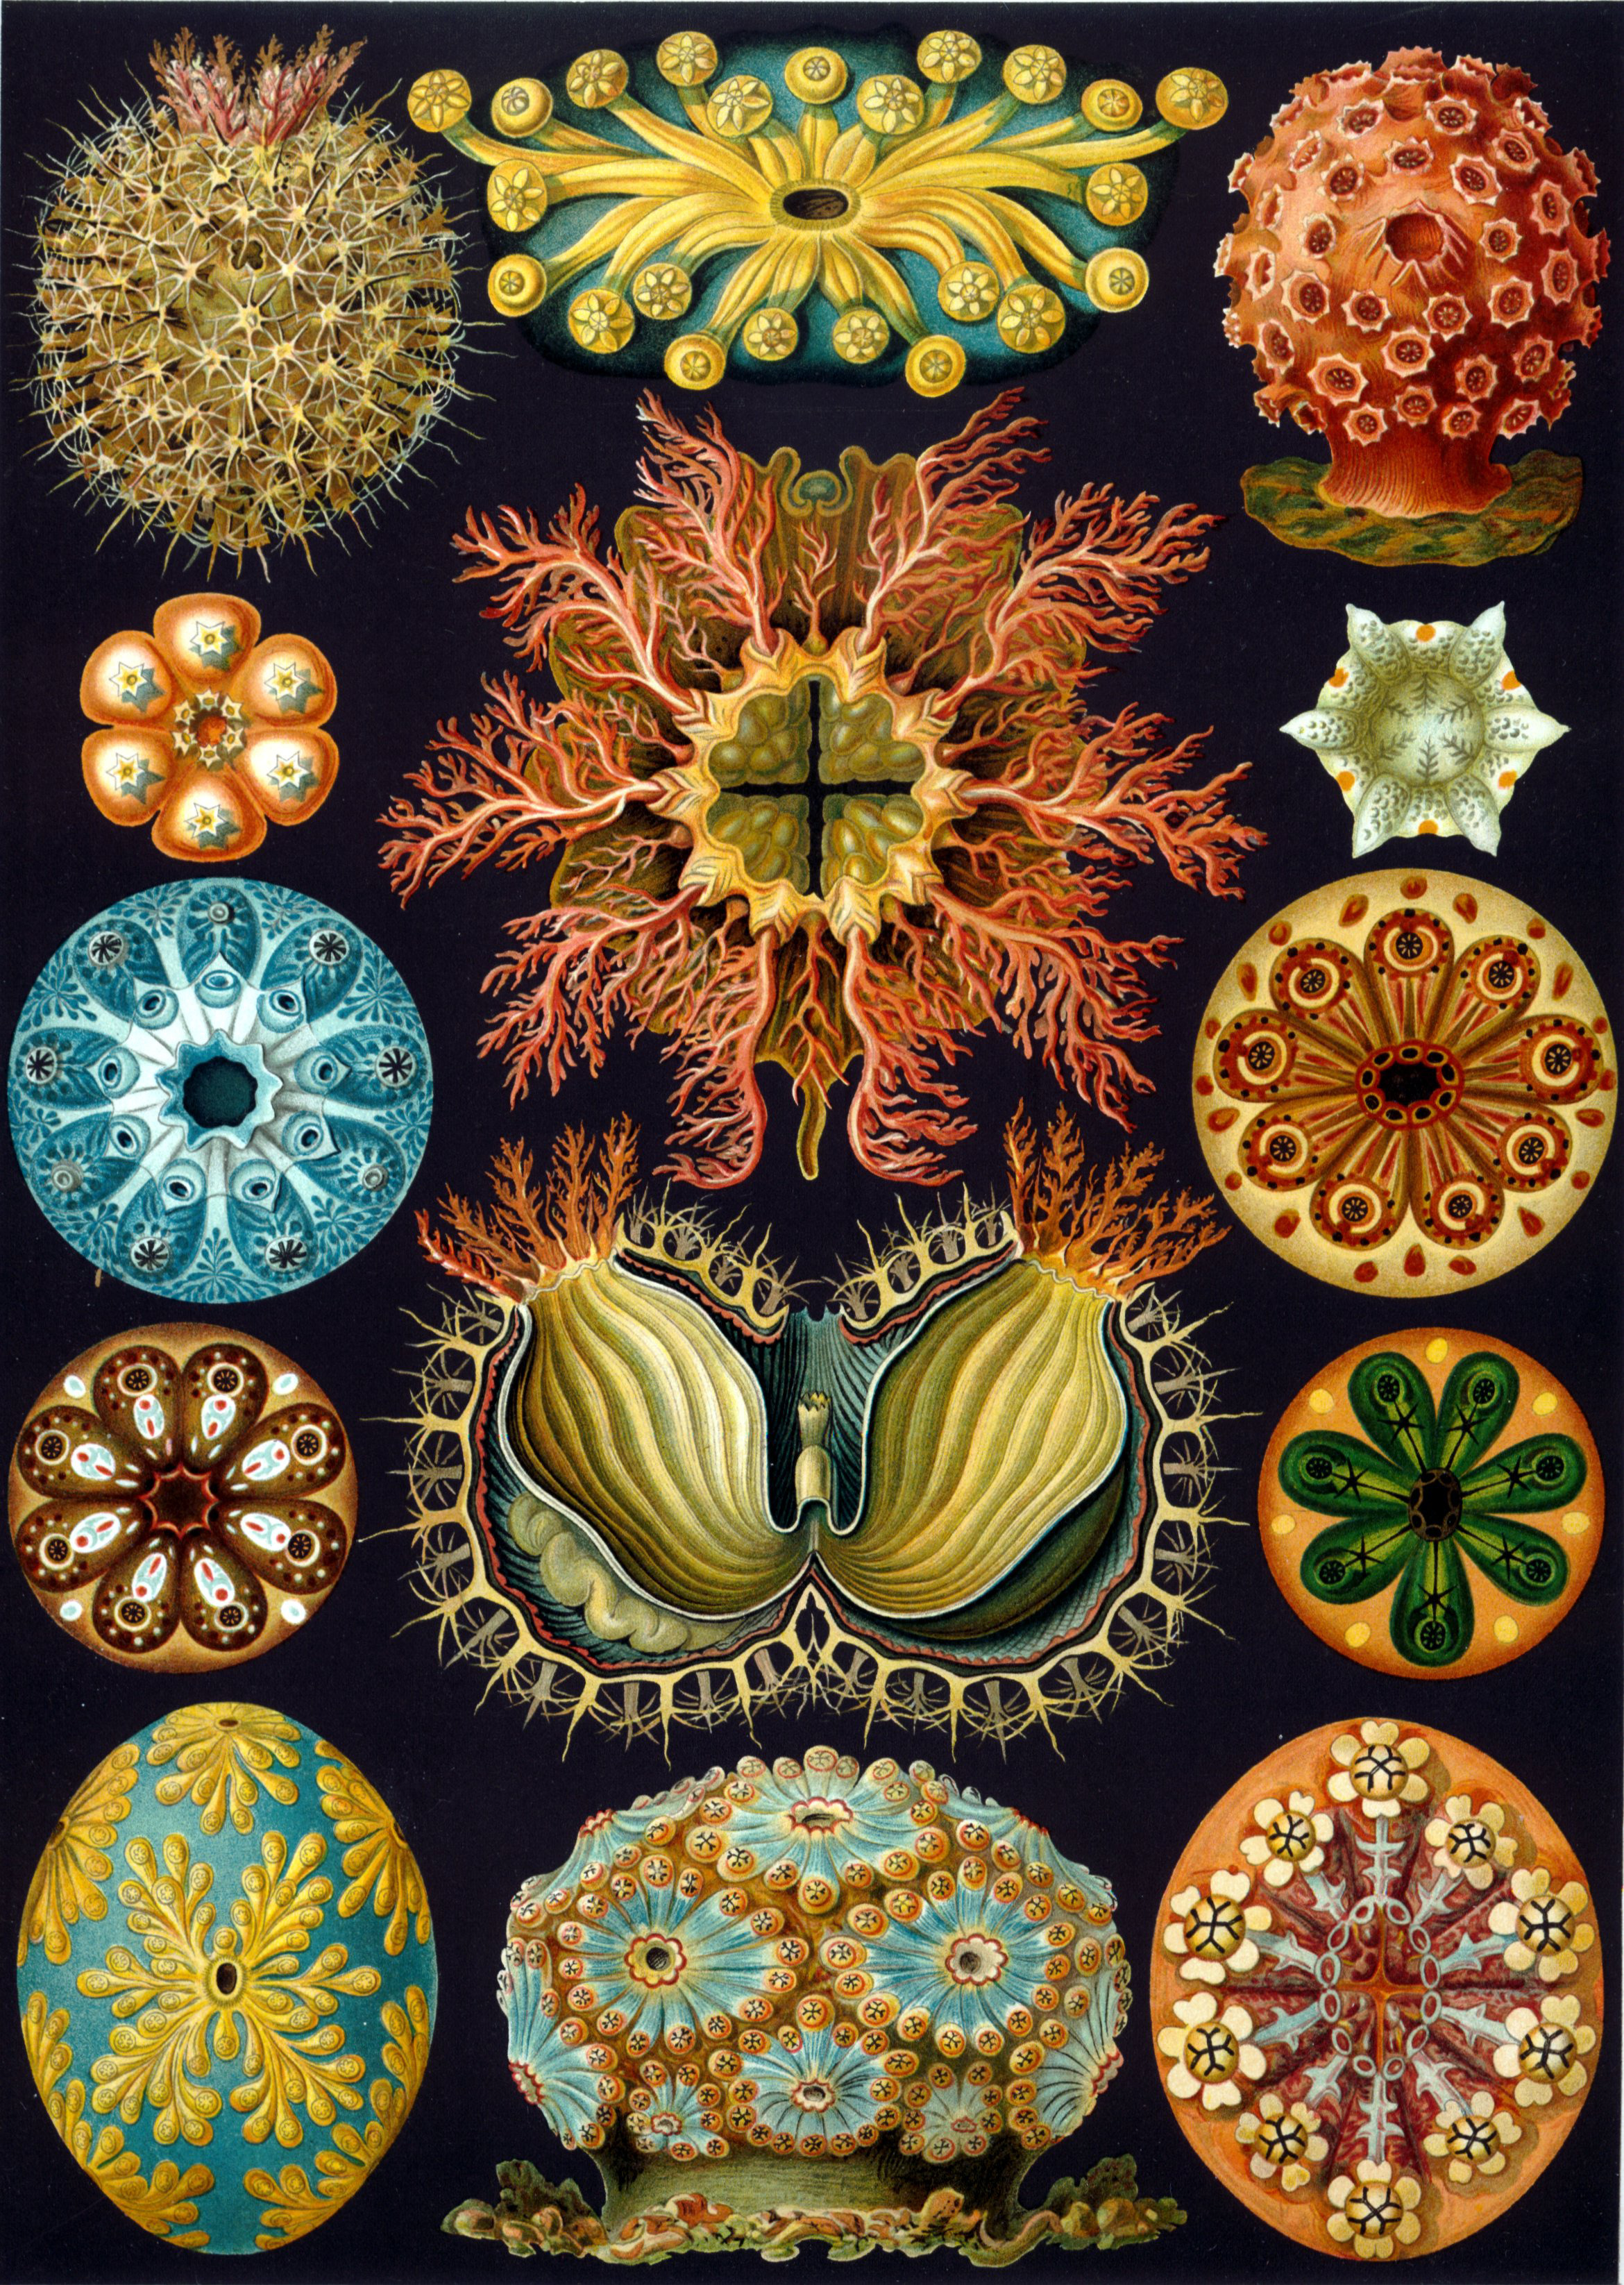
\includegraphics[width=0.7\linewidth]{./figures/echinodermata/Haeckel_Ascidiae}

}

\caption{\href{https://commons.wikimedia.org/wiki/File:Haeckel_Ascidiae.jpg}{Ascidians}}\label{fig:ascidians}
\end{figure}

\section{View Prepared Slides of
Tunicates}\label{view-prepared-slides-of-tunicates}

\begin{enumerate}
\def\labelenumi{\arabic{enumi}.}
\tightlist
\item
  \href{https://en.wikipedia.org/wiki/Ascidiacea}{\emph{Ascidian}} larva
  w.m. (Figure \ref{fig:ascidian})

  \begin{itemize}
  \tightlist
  \item
    Identify: notochord
  \end{itemize}
\end{enumerate}

\begin{figure}

{\centering 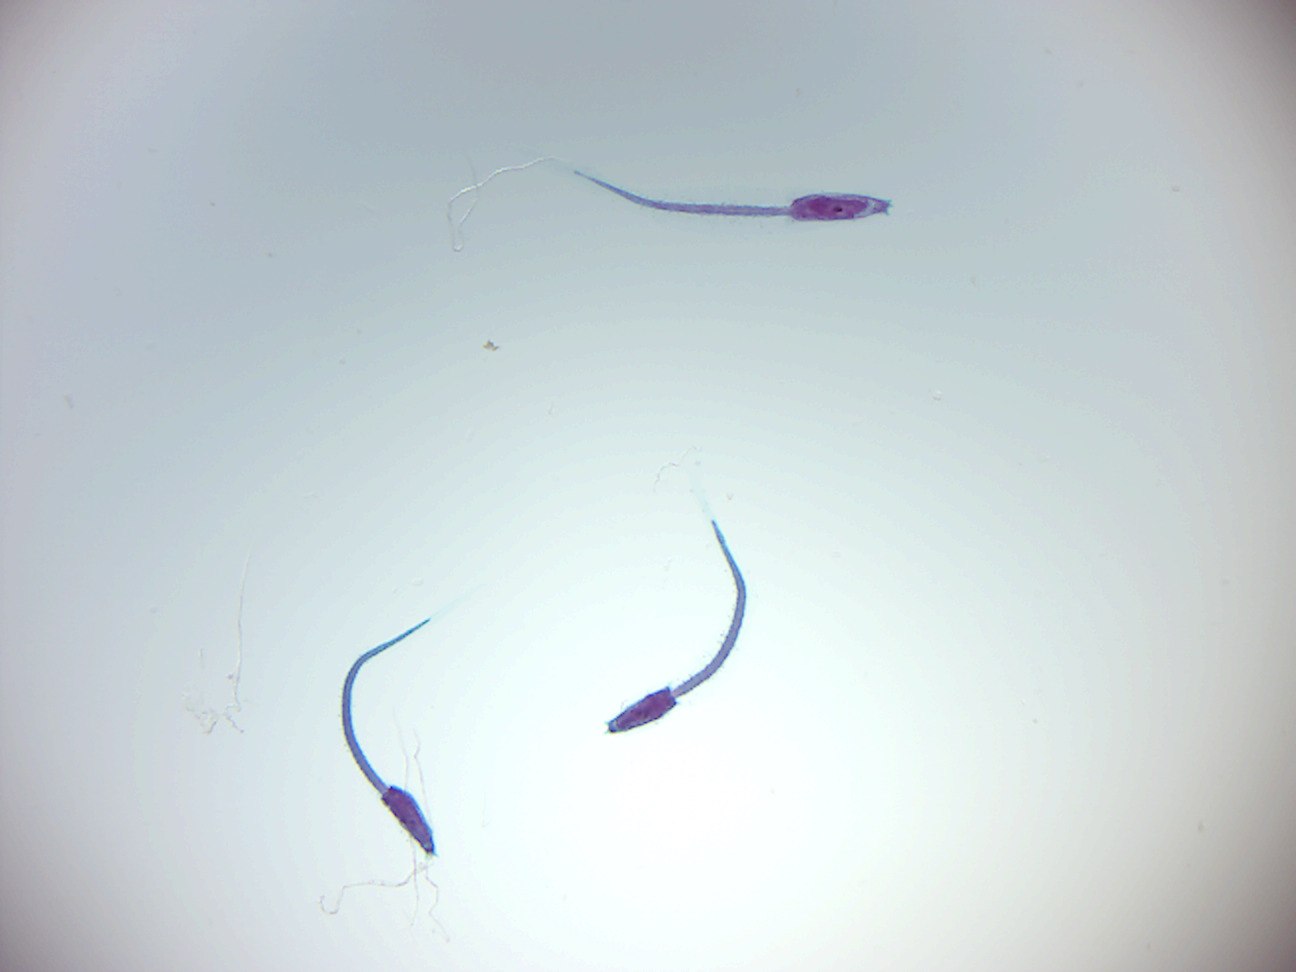
\includegraphics[width=0.7\linewidth]{./figures/echinodermata/ascidian_larva}

}

\caption{Ascician larva.}\label{fig:ascidian}
\end{figure}

\section{Cephalochordates}\label{cephalochordates}

Cephalochordates are small, ``vaguely fish-shaped'' animals that lack
brains, clearly defined heads and specialized sense organs. These
burrowing filter-feeders compose the earliest-branching chordate
sub-phylum.

\href{https://en.wikipedia.org/wiki/Lancelet}{Lancelet} (Amphioxus)
\emph{Branchiostoma lanceolatum} (European lancelet) is a lancelet in
the subphylum Cephalochordata. It is a marine invertebrate with a
notochord but no backbone and is used as a model organism to study the
evolutionary development of vertebrates.

Is found in shallow seas in the north-east Atlantic Ocean, from Norway,
Scotland as well as further south to the Mediterranean Sea and the Black
Sea. Its range has expanded through the Suez Canal to the northerly
parts of the Indian Ocean and the coasts of East Africa. It burrows in
soft substrates such as sand, gravel and shell fragments and is quite
particular as to the size of the particles. It occurs from the low tide
mark down to about 40 meters.

It has an elongated body, flattened laterally and pointed at both ends.
A stiffening rod of tightly packed cells, the notochord, extends the
whole length of the body. Above it is a nerve cord with a single frontal
eye. The mouth is on the underside of the body and is surrounded by a
tuft of 20 or 30 cirri or slender sensory appendages. The gut runs just
below the notochord from the mouth to the anus, in front of the tail.
There is a flap-like, vertical fin surrounding the pointed tail. Gas
exchange takes place as water passes through gill slits in the mid
region, and segmented gonads lie just behind these. The animal is pearly
white and semi-transparent which enables the internal organs to be seen
from outside. Its appearance is similar to a ``primitive fish''. It can
grow up to 6 cm.

\section{View Prepared Slides of
Lancelet}\label{view-prepared-slides-of-lancelet}

\begin{enumerate}
\def\labelenumi{\arabic{enumi}.}
\tightlist
\item
  Lancelet w.m. (Figure \ref{fig:lanceletwm})

  \begin{itemize}
  \tightlist
  \item
    Locate: dorsal hollow nerve cord, notochord, pharyngeal gill slit,
    buccal cavity, buccal cirri (oral tentacles), atriopore, anus,
    liver, myotomes, post-anal tail.
  \end{itemize}
\item
  Lancelet x.s. through pharynx (Figure \ref{fig:lanceletxs})

  \begin{itemize}
  \tightlist
  \item
    Locate: dorsal hollow nerve cord, notochord, pharyngeal gill slits,
    myotomes, liver.
  \end{itemize}
\end{enumerate}

\begin{figure}

{\centering 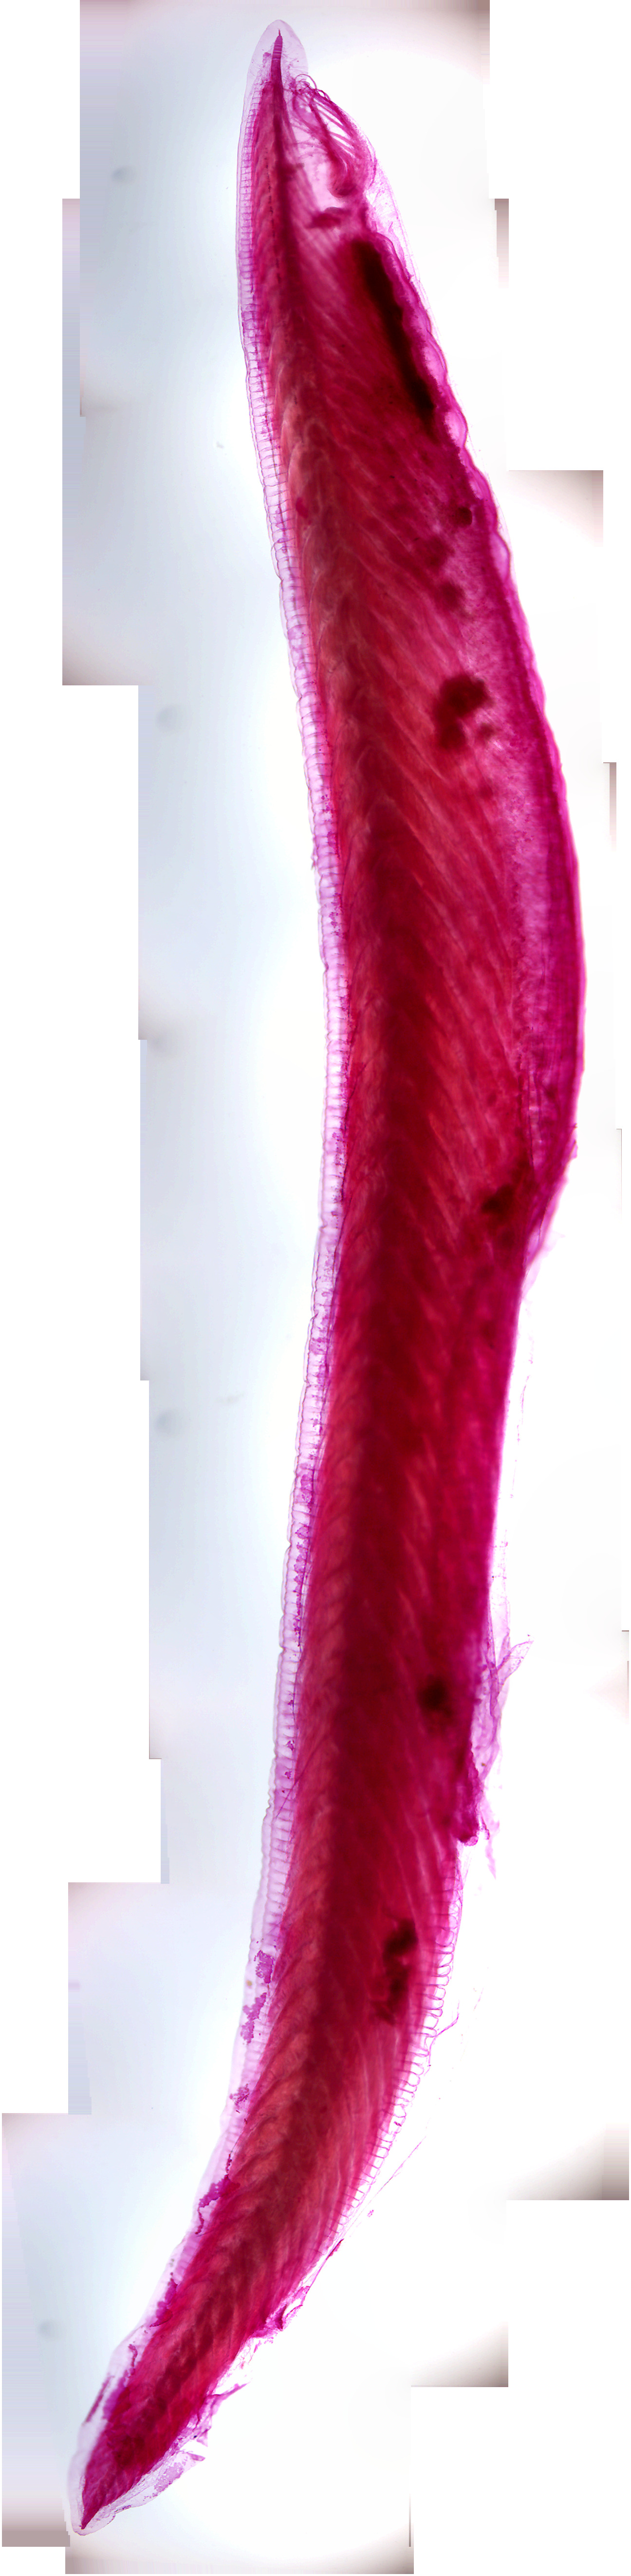
\includegraphics[width=0.7\linewidth]{./figures/echinodermata/lancelet_wm}

}

\caption{A young adult lancelet.}\label{fig:lanceletwm}
\end{figure}

\begin{figure}

{\centering 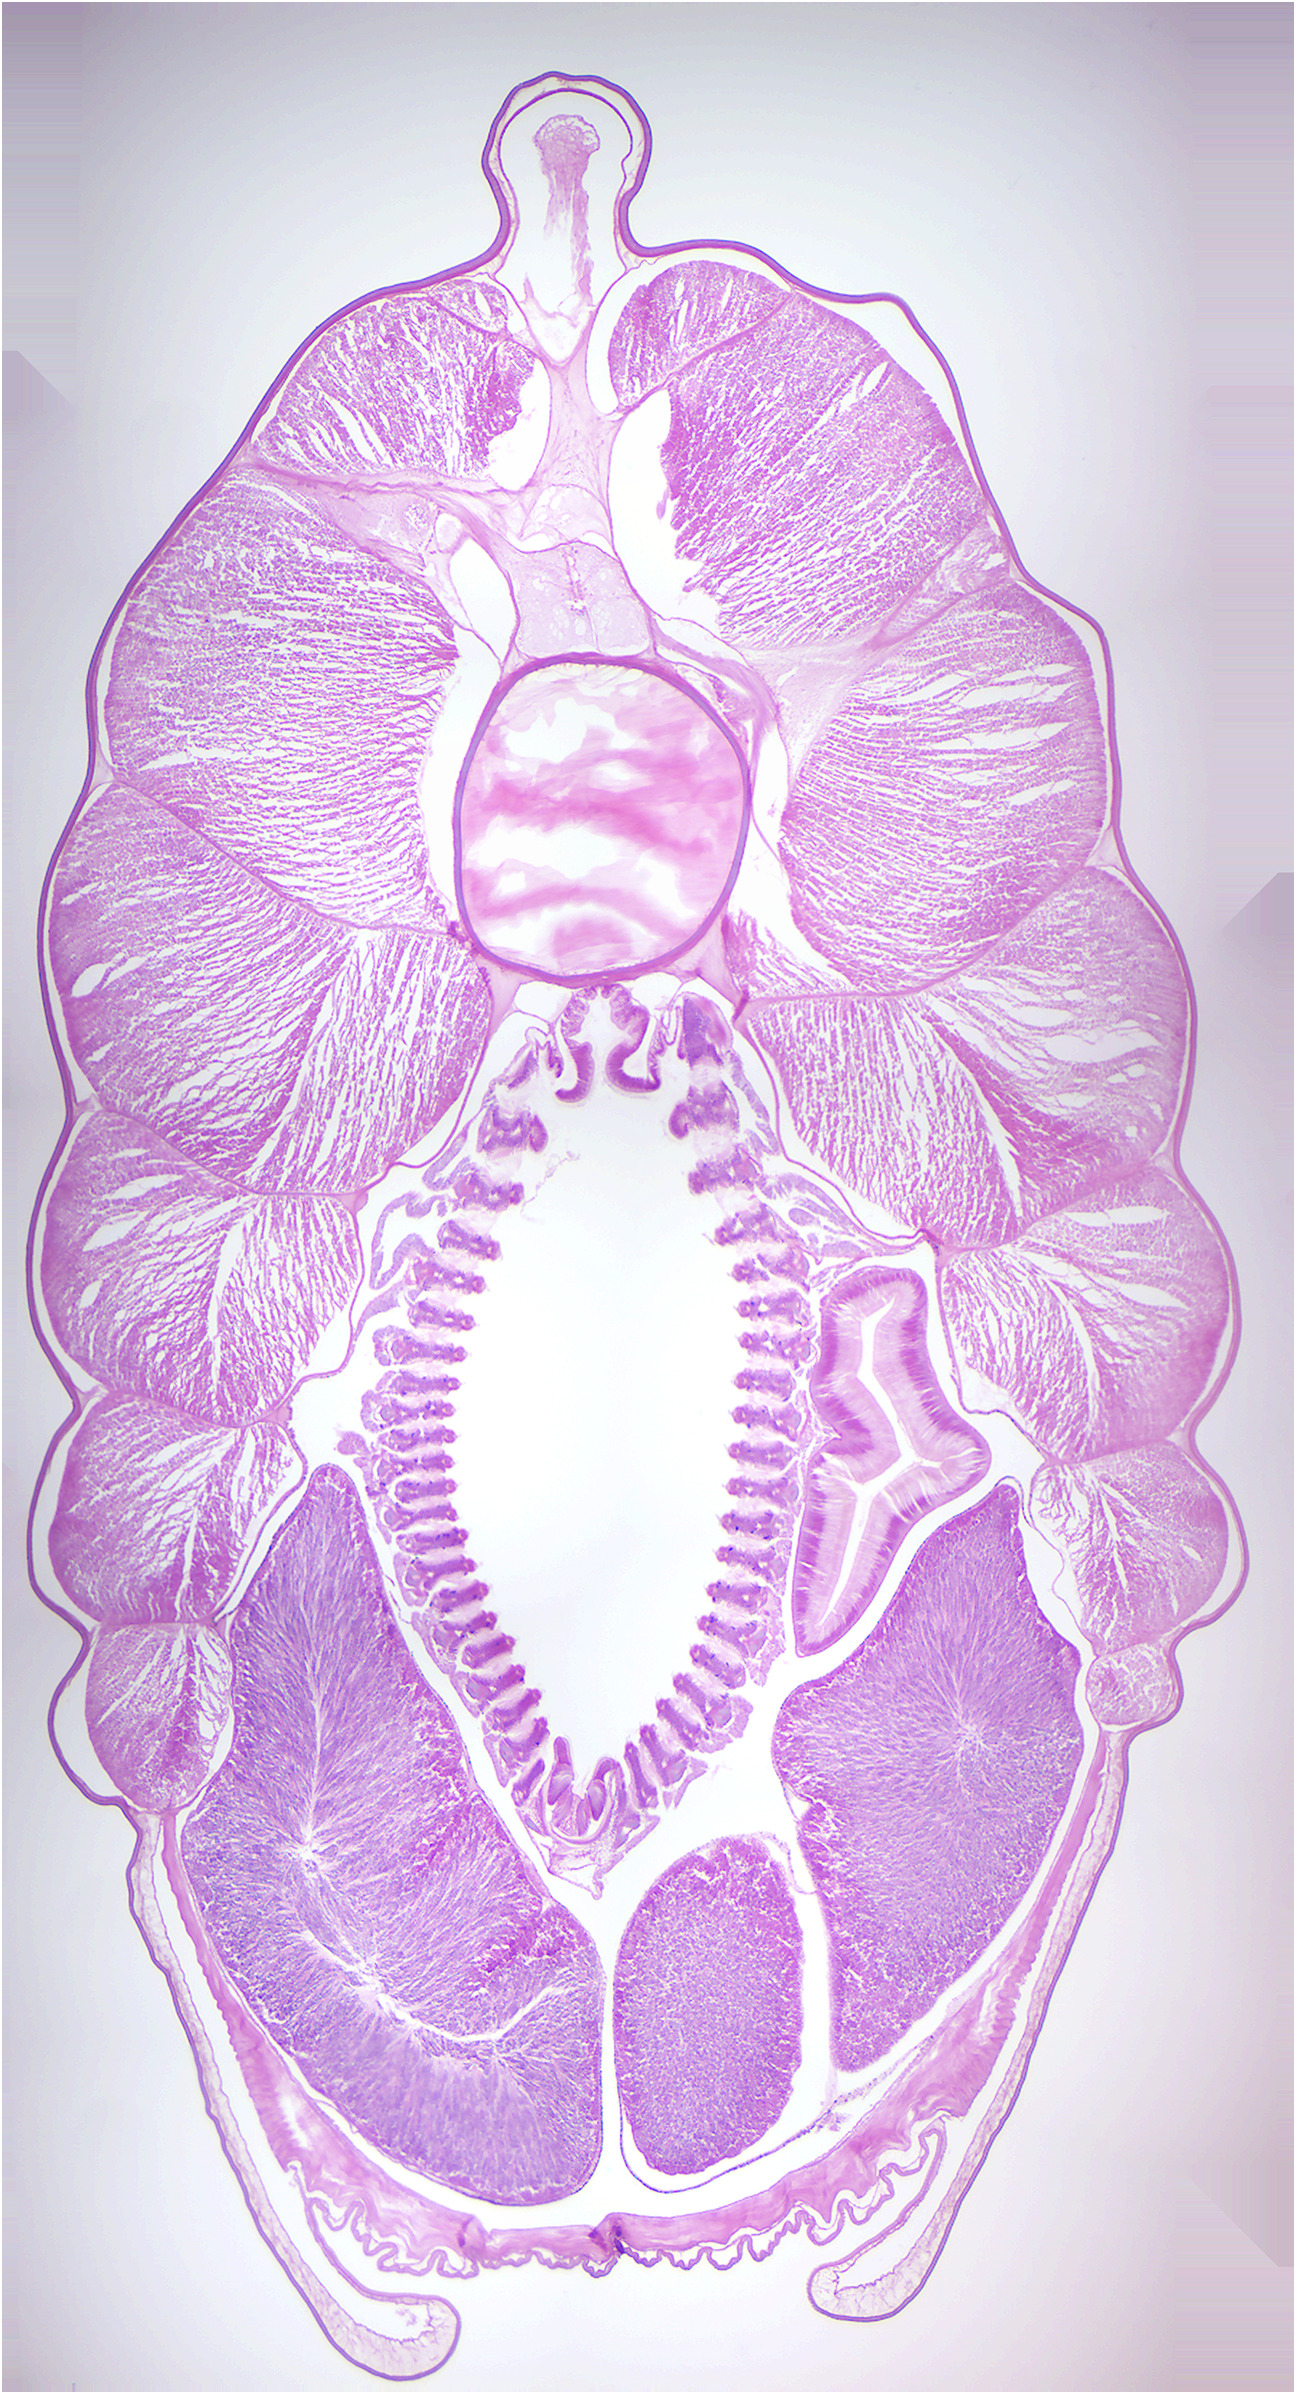
\includegraphics[width=0.7\linewidth]{./figures/echinodermata/lancelet_xs}

}

\caption{Lancelet cross section.}\label{fig:lanceletxs}
\end{figure}

\section{Review Questions}\label{review-questions-6}

\begin{enumerate}
\def\labelenumi{\arabic{enumi}.}
\tightlist
\item
  What are echinoderms?
\item
  What are tube feet?
\item
  What the five characteristics of chordates?
\item
  What is the notochord?
\item
  What are tunicates?
\end{enumerate}
